%%%%%%%%%%%%%%%%%%%%%%%%%%%%%%%%%%%%% BEGIN HEADERS %%%%%%%%%%%%%%%%%%%%%%%%%%%%%%%%%%%%%%%%%%%%%%%%%%%%%
\documentclass[11pt,conference]{IEEEtran}

\usepackage{longtable}
\usepackage{graphicx}
\usepackage[utf8]{inputenc}
\usepackage{fancyhdr}
\usepackage{float}
\usepackage[hidelinks]{hyperref}
\usepackage{listings}
\usepackage{color}
\usepackage{natbib}
\usepackage{caption}

% Your names in the header
\pagestyle{fancy}
\rhead{Enrico Tedeschi, Mike Murphy}
\lhead{INF-3200 Distributed Systems - Assignment 2}
\cfoot{\thepage}

% Used for including code in a stylized manner
\definecolor{codegreen}{rgb}{0,0.6,0}
\definecolor{codegray}{rgb}{0.5,0.5,0.5}
\definecolor{codepurple}{rgb}{0.58,0,0.82}
\definecolor{backcolour}{rgb}{0.95,0.95,0.92}
 

\lstdefinestyle{mystyle}{
    backgroundcolor=\color{backcolour},   
    commentstyle=\color{codegreen},
    keywordstyle=\color{magenta},
    numberstyle=\tiny\color{codegray},
    stringstyle=\color{codepurple},
    basicstyle=\footnotesize,
    breakatwhitespace=false,         
    breaklines=true,                 
    captionpos=b,                    
    keepspaces=true,                 
    numbers=left,                    
    numbersep=5pt,                  
    showspaces=false,                
    showstringspaces=false,
    showtabs=false,                  
    tabsize=2
}

\lstset{style=mystyle}

% The Title
\title{UiT INF-3200 Distributed Systems - Project 2\\Fall 2015}

% Your name and email
\author{Enrico Tedeschi\\ete011@post.uit.no
    \and Mike Murphy\\mmu019@post.uit.no}


%%%%%%%%%%%%%%%%%%%%%%%%%%%%%%%%%%%%% END HEADERS %%%%%%%%%%%%%%%%%%%%%%%%%%%%%%%%%%%%%%%%%%%%%%%%%%%%%

\begin{document}

% Create the title and everything
\maketitle


\section{Introduction}

Our task was to implement leader election on top of a peer-to-peer network.

All the peers in the network must agree on who the leader is and only one peer can be leader at a time. Provides support for peers joining and leaving the network.


\subsection{Requirements}

\begin{itemize}
\item Support at least 10 nodes in a p2p network structure of your own choice. No centralized architectures allowed; i.e. all processes should behave similarly.
\item Support graceful shutdown of nodes. On receiving a signal to shut down(SIGTERM), a node should leave the network.
\item Support adding nodes on demand. Adding a new process allows you to grow the system as the demand increases.
\item Leader election. There should at all times be a single leader. A pertinent Q: What happens if the leader leaves the network?
\item A GET request to any node for the url "/getCurrentLeader" should return the ip and port of the current leader. The response body must be formatted as a single ip:port (e.g. "127.0.0.1:1234") entry.
\item A GET request to any node for the url "/getNodes" should return a list of ip and port pairs of all nodes connected to the recipent node. The response body must be formatted as a list of ip:port (e.g. "127.0.0.1:1234") entries with newline separating each ip:port pair.
\item Measure the time it takes to elect a leader when the number of nodes changes.
\end{itemize}


\section{Technical Background}
To solve the problem some technical background are required. First of all, a good knowledge about programming and some basic concept about distributed systems is necessary. Is good to know and to study then, some of the possible election algorithms which could be used. We took into consideration the \textit{Bully algorithm} and the \textit{Ring algorithm election}.

\subsection{Bully algorithm}
When a new leader is needed a process \textit{P} send an election message to all the nodes with an higher ID number. If there are no answers, \textit{P} wins the election. If \textit{P} gets an answer then it terminates his job and the election continues with the node with the higher value just called. In the Fig \ref{fig:bully} the node 3 starts the election because the previous leader 6 crashed. The new leader will be the node 5.
\begin{figure}[h!]
  \centering
    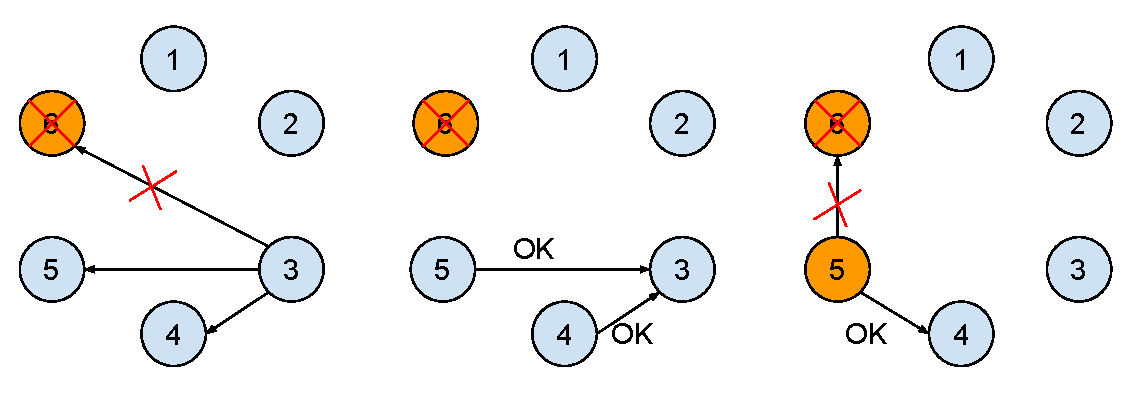
\includegraphics[width=0.5\textwidth]{bully}
    \caption{Example of how the bully algorithm works, the leader changes from 6 to 5}
    \label{fig:bully}
\end{figure}

\subsection{Ring algorithm election}
Every node needs to know only about his successor. When any process figures out that there is no leader anymore, it generates an election message. The message flows through the ring network and every node adds its ID in it. If a node finds its ID in the message it means that that node started the election, so it will be the new leader and a new message will be sent to announce the new coordinator. In the Fig \ref{fig:ring} the node 5 realize that the coordinator is down. It start a new election and at the end it gets the leader role. Then it sends an ok message which tells to the other nodes who is the new coordinator.
\begin{figure}[h!]
  \centering
    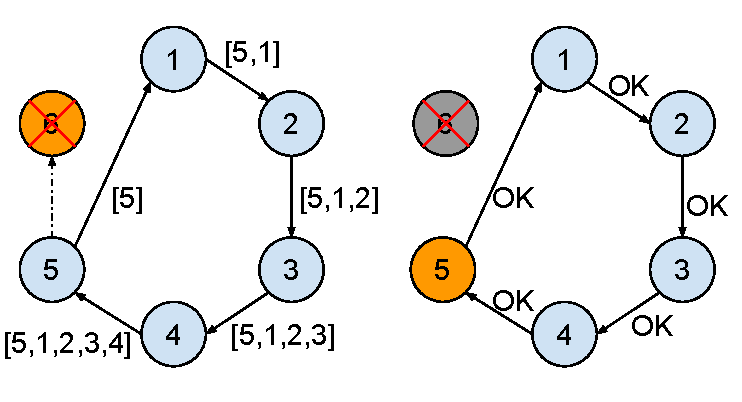
\includegraphics[width=0.5\textwidth]{ring}
    \caption{Example of how the ring algorithm election works, the leader changes from node 6 to node 5, the election is started from the node 5}
    \label{fig:ring}
\end{figure}
%TODO: talk about leader, algorithm election, and problems in joining and leaving

\section{Design}

%TODO: talk about the ring design and which one was chosen in the implementation

\section{Implementation}

%TODO: talk about why the ring algorithm was chosen (because from the previous version of the implemented network each node has information about his successor -- which is required for the ring algorithm)

\subsection{Languages and Code}

Our solution is implemented in a mix of Python and Bash script, Python for the
actual node implementation, and a Bash script to communicate through the network created, adding and removing nodes.

We started with skeleton code by our first assignment for what concerns the node and the script code. 
The code was rearranged by removing the front-end node and by adding some properties to the nodes such as the predecessor node and information about the leader, which at the beginning, is the first node joining the network.

The code were tested before on local machine, using bash scripts and the given visual test code from Einar Holsbø Jakobsen and Magnus Stenhaug and then on the uvrocks cluster.

\subsection{Network Protocol}




\subsection{Persistence}




\subsection{Frontend}




\subsection{Node}



\subsection{Environment}

Our code was written to run on the Rocks Cluster distribution\cite{rocks}, and
makes some assumptions about that environment. We rely on the cluster's shared
filesystem for distributing program code to servers. And we rely on easy SSH
access between machines in the cluster to start and shutdown nodes.


\section{Discussion}

%TODO: Talk about why was chosen the ring design over the bully (bully maybe faster because the messages are sent only through the nodes with an higher ID). Consider also the case in which two nodes realize that the leader is missing. Talk about the graceful shutdown so there will be no problem in just know the successor since we won't manage crashes.


\section{Evaluation}
For the evaluation node scaling has been considered. The function \textit{storage\_frontend} has been timed sending five hundred requests (GET/PUT) to the nodes network. The evaluation has been done considering the scale on the number of nodes and for each, 10 tests were taken into consideration.
\newline
The number of nodes and the average time of 10 computations is represented in the table in Fig \ref{tab:scaling}.

\begin{figure}[h!]
\centering
% \renewcommand{\figurename}{Fig.}
\caption{Nodes/Time scaling table}
\begin{tabular}[H]{ | l | l | }
\hline
	Nodes & Time \\ \hline
	2 & 5.7923 \\ \hline
	4 & 6.4793 \\ \hline
	6 & 8.1309 \\ \hline
	10 & 13.0746 \\ \hline
	15 & 17.0469 \\ \hline
	20 & 19.3472 \\ \hline
	30 & 29.4729 \\ \hline
	40 & 35.2886 \\ \hline
\end{tabular}
\label{tab:scaling}
\end{figure}

In the Fig \ref{fig:scaling} instead the graphic of this scaling test is characterized.




\section{Conclusion}

Our DHT solution, with a simple ring structure, was able to store and retrieve
data correctly, in time that increased linearly with the number of nodes
($O(n)$).


\bibliographystyle{plain}
\bibliography{report}


\end{document}
